\documentclass{article}
\usepackage{tikz}
\usetikzlibrary{mindmap}

\begin{document}

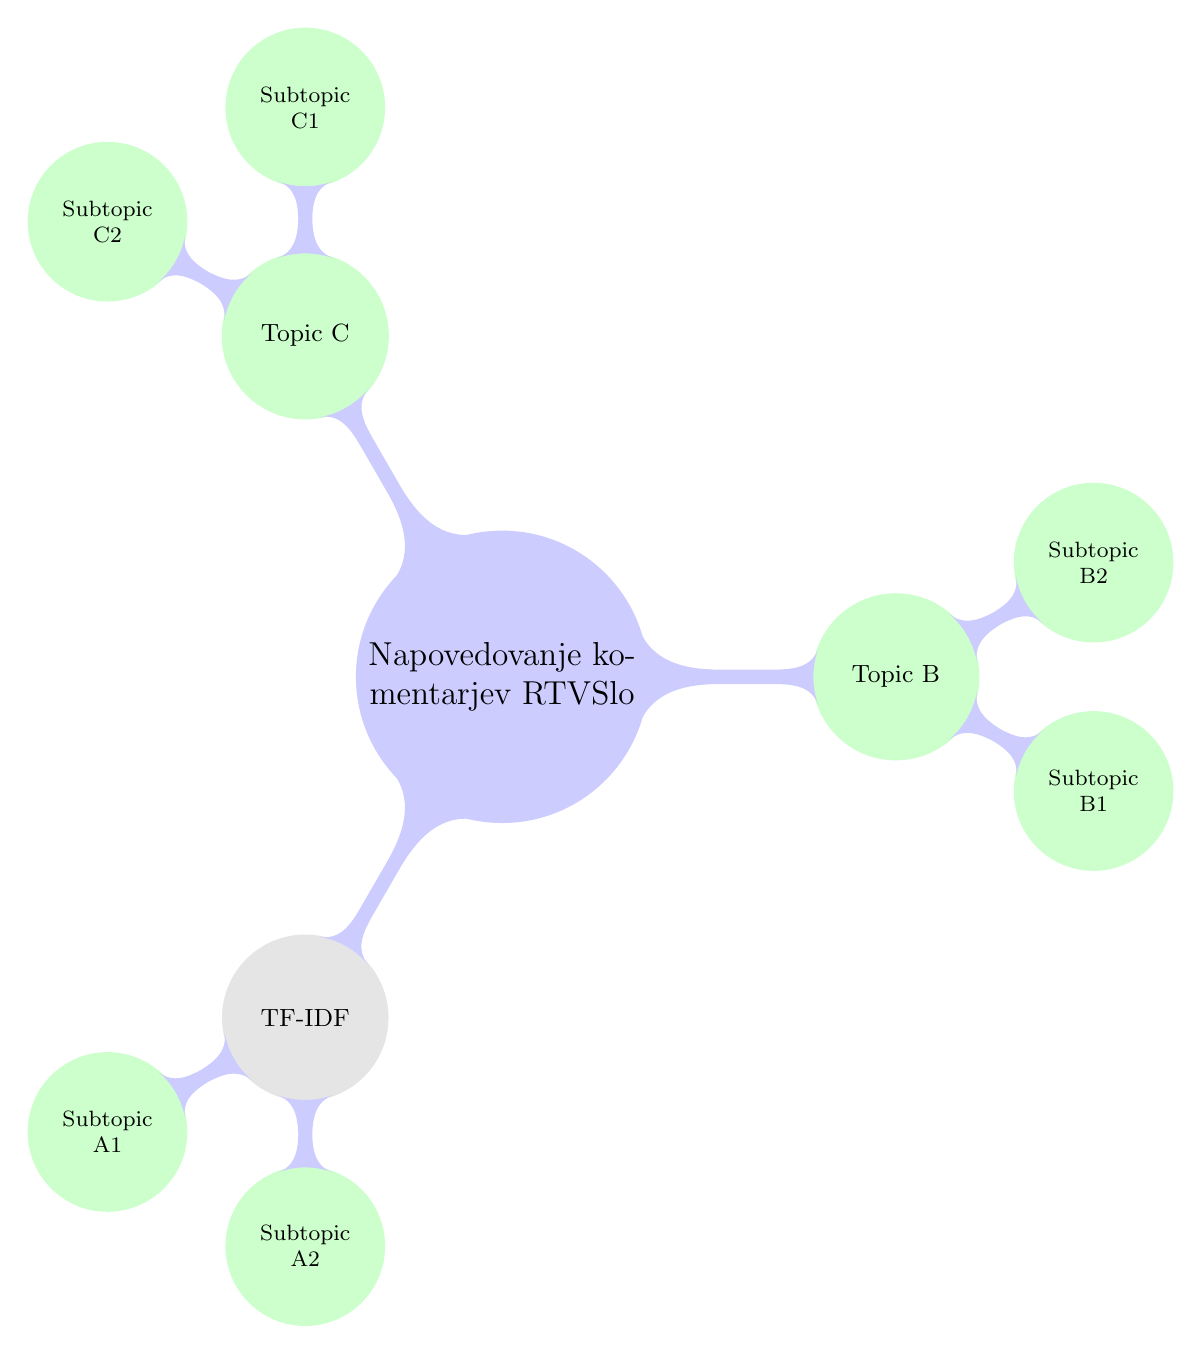
\begin{tikzpicture}[mindmap,
    every node/.style={concept, draw, circle, thick, text=black, minimum size=2cm},
    concept color=blue!20,
    grow cyclic,
    level 1/.append style={sibling angle=120},
    level 2/.append style={sibling angle=60},
    ]
  \node {Napovedovanje komentarjev RTVSlo}
      child { node[concept color=gray!20] {TF-IDF}
          child { node[concept color=green!20] {Subtopic A1} }
          child { node[concept color=green!20] {Subtopic A2} }
        }
      child { node[concept color=green!20] {Topic B}
          child { node[concept color=green!20] {Subtopic B1} }
          child { node[concept color=green!20] {Subtopic B2} }
        }
      child { node[concept color=green!20] {Topic C}
          child { node[concept color=green!20] {Subtopic C1} }
      child { node[concept color=green!20] {Subtopic C2} }
    };
\end{tikzpicture}

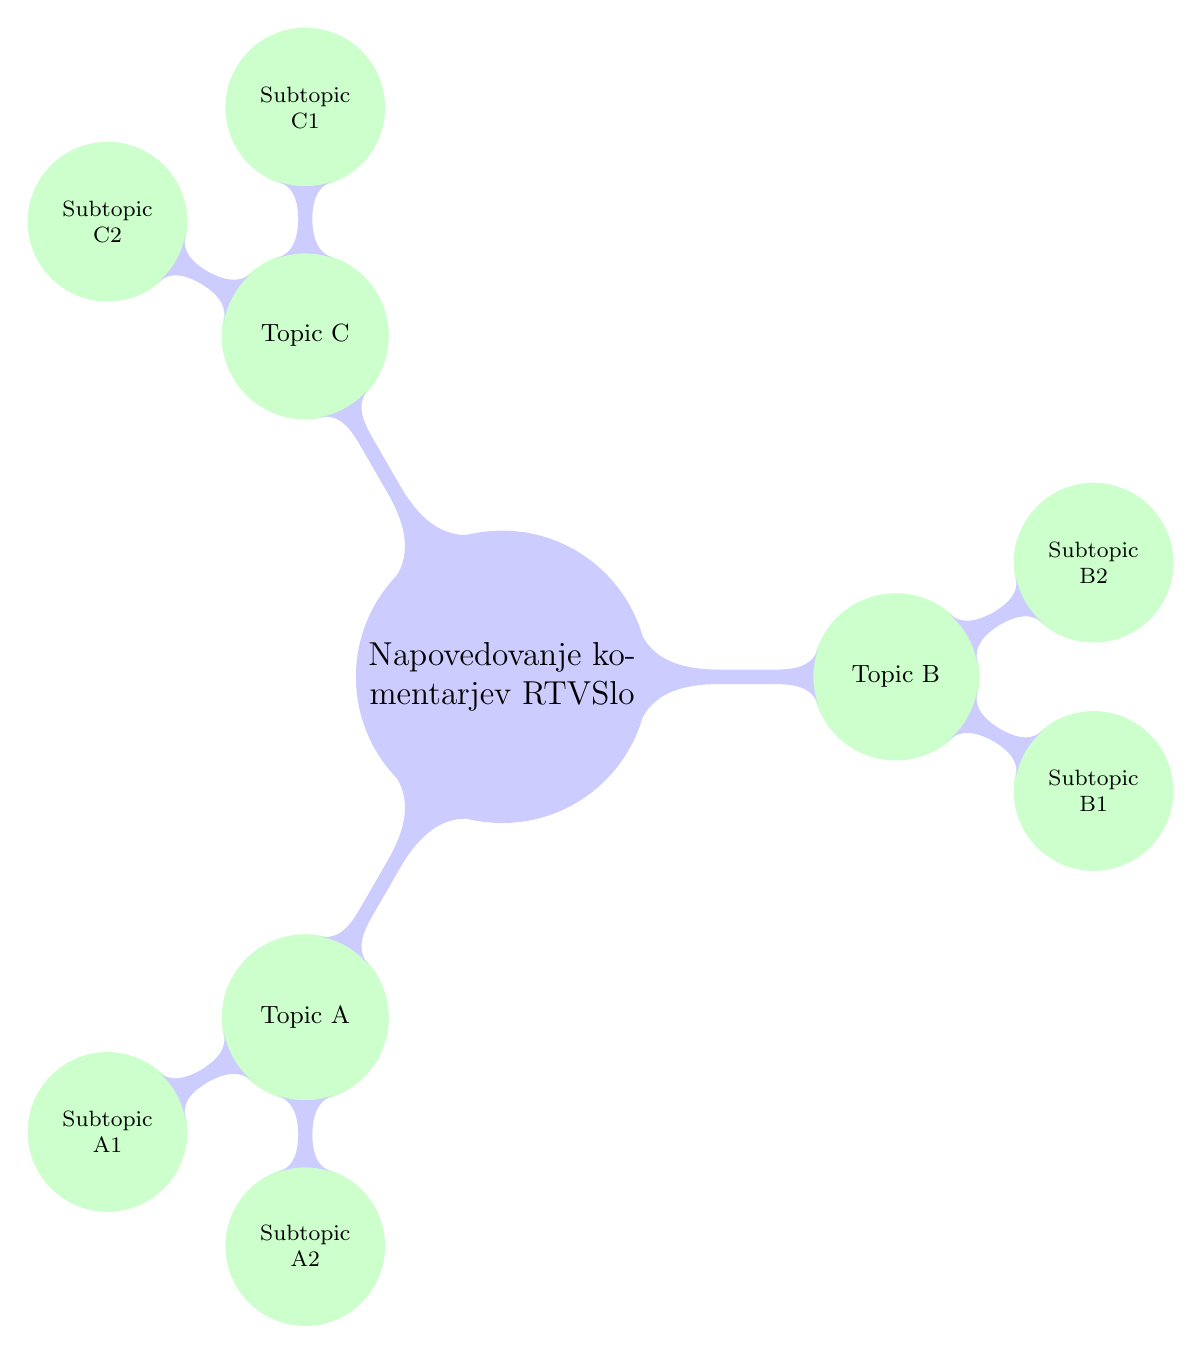
\begin{tikzpicture}[mindmap,
    every node/.style={concept, draw, circle, thick, text=black, minimum size=2cm},
    concept color=blue!20,
    grow cyclic,
    level 1/.append style={sibling angle=120},
    level 2/.append style={sibling angle=60},
    ]
  \node {Napovedovanje komentarjev RTVSlo}
      child { node[concept color=green!20] {Topic A}
      child { node[concept color=green!20] {Subtopic A1} }
      child { node[concept color=green!20] {Subtopic A2} }
    }
    child { node[concept color=green!20] {Topic B}
      child { node[concept color=green!20] {Subtopic B1} }
      child { node[concept color=green!20] {Subtopic B2} }
    }
    child { node[concept color=green!20] {Topic C}
      child { node[concept color=green!20] {Subtopic C1} }
      child { node[concept color=green!20] {Subtopic C2} }
    };
\end{tikzpicture}


\end{document}

